% camera ready
\pagebreak
\section{GUI Setup and Demonstration}
\label{section_gui}

Following contains the steps to set up the GUI
\begin{enumerate}
  \item Clone the Github repository \newline \verb|git clone https://github.com/tinkitwong/kaggle-environments|.
  \item Navigate into directory of the repository
  \item Create a python Virtual Environment \verb|python3 -m venv env|
  \item Activate Virtual Environment \verb|source env/bin/activate|
  \item Install Dependencies \verb|pip install requirements.txt|
  \item Start the Jupyter server \verb|./env/bin/jupyter notebook|
  \item Navigate into notebook \verb|playtest.ipynb|
  \item Run the first two cells of the notebook (Figure \ref{figure_controls})
\end{enumerate}

\begin{figure}[!h]
\centering
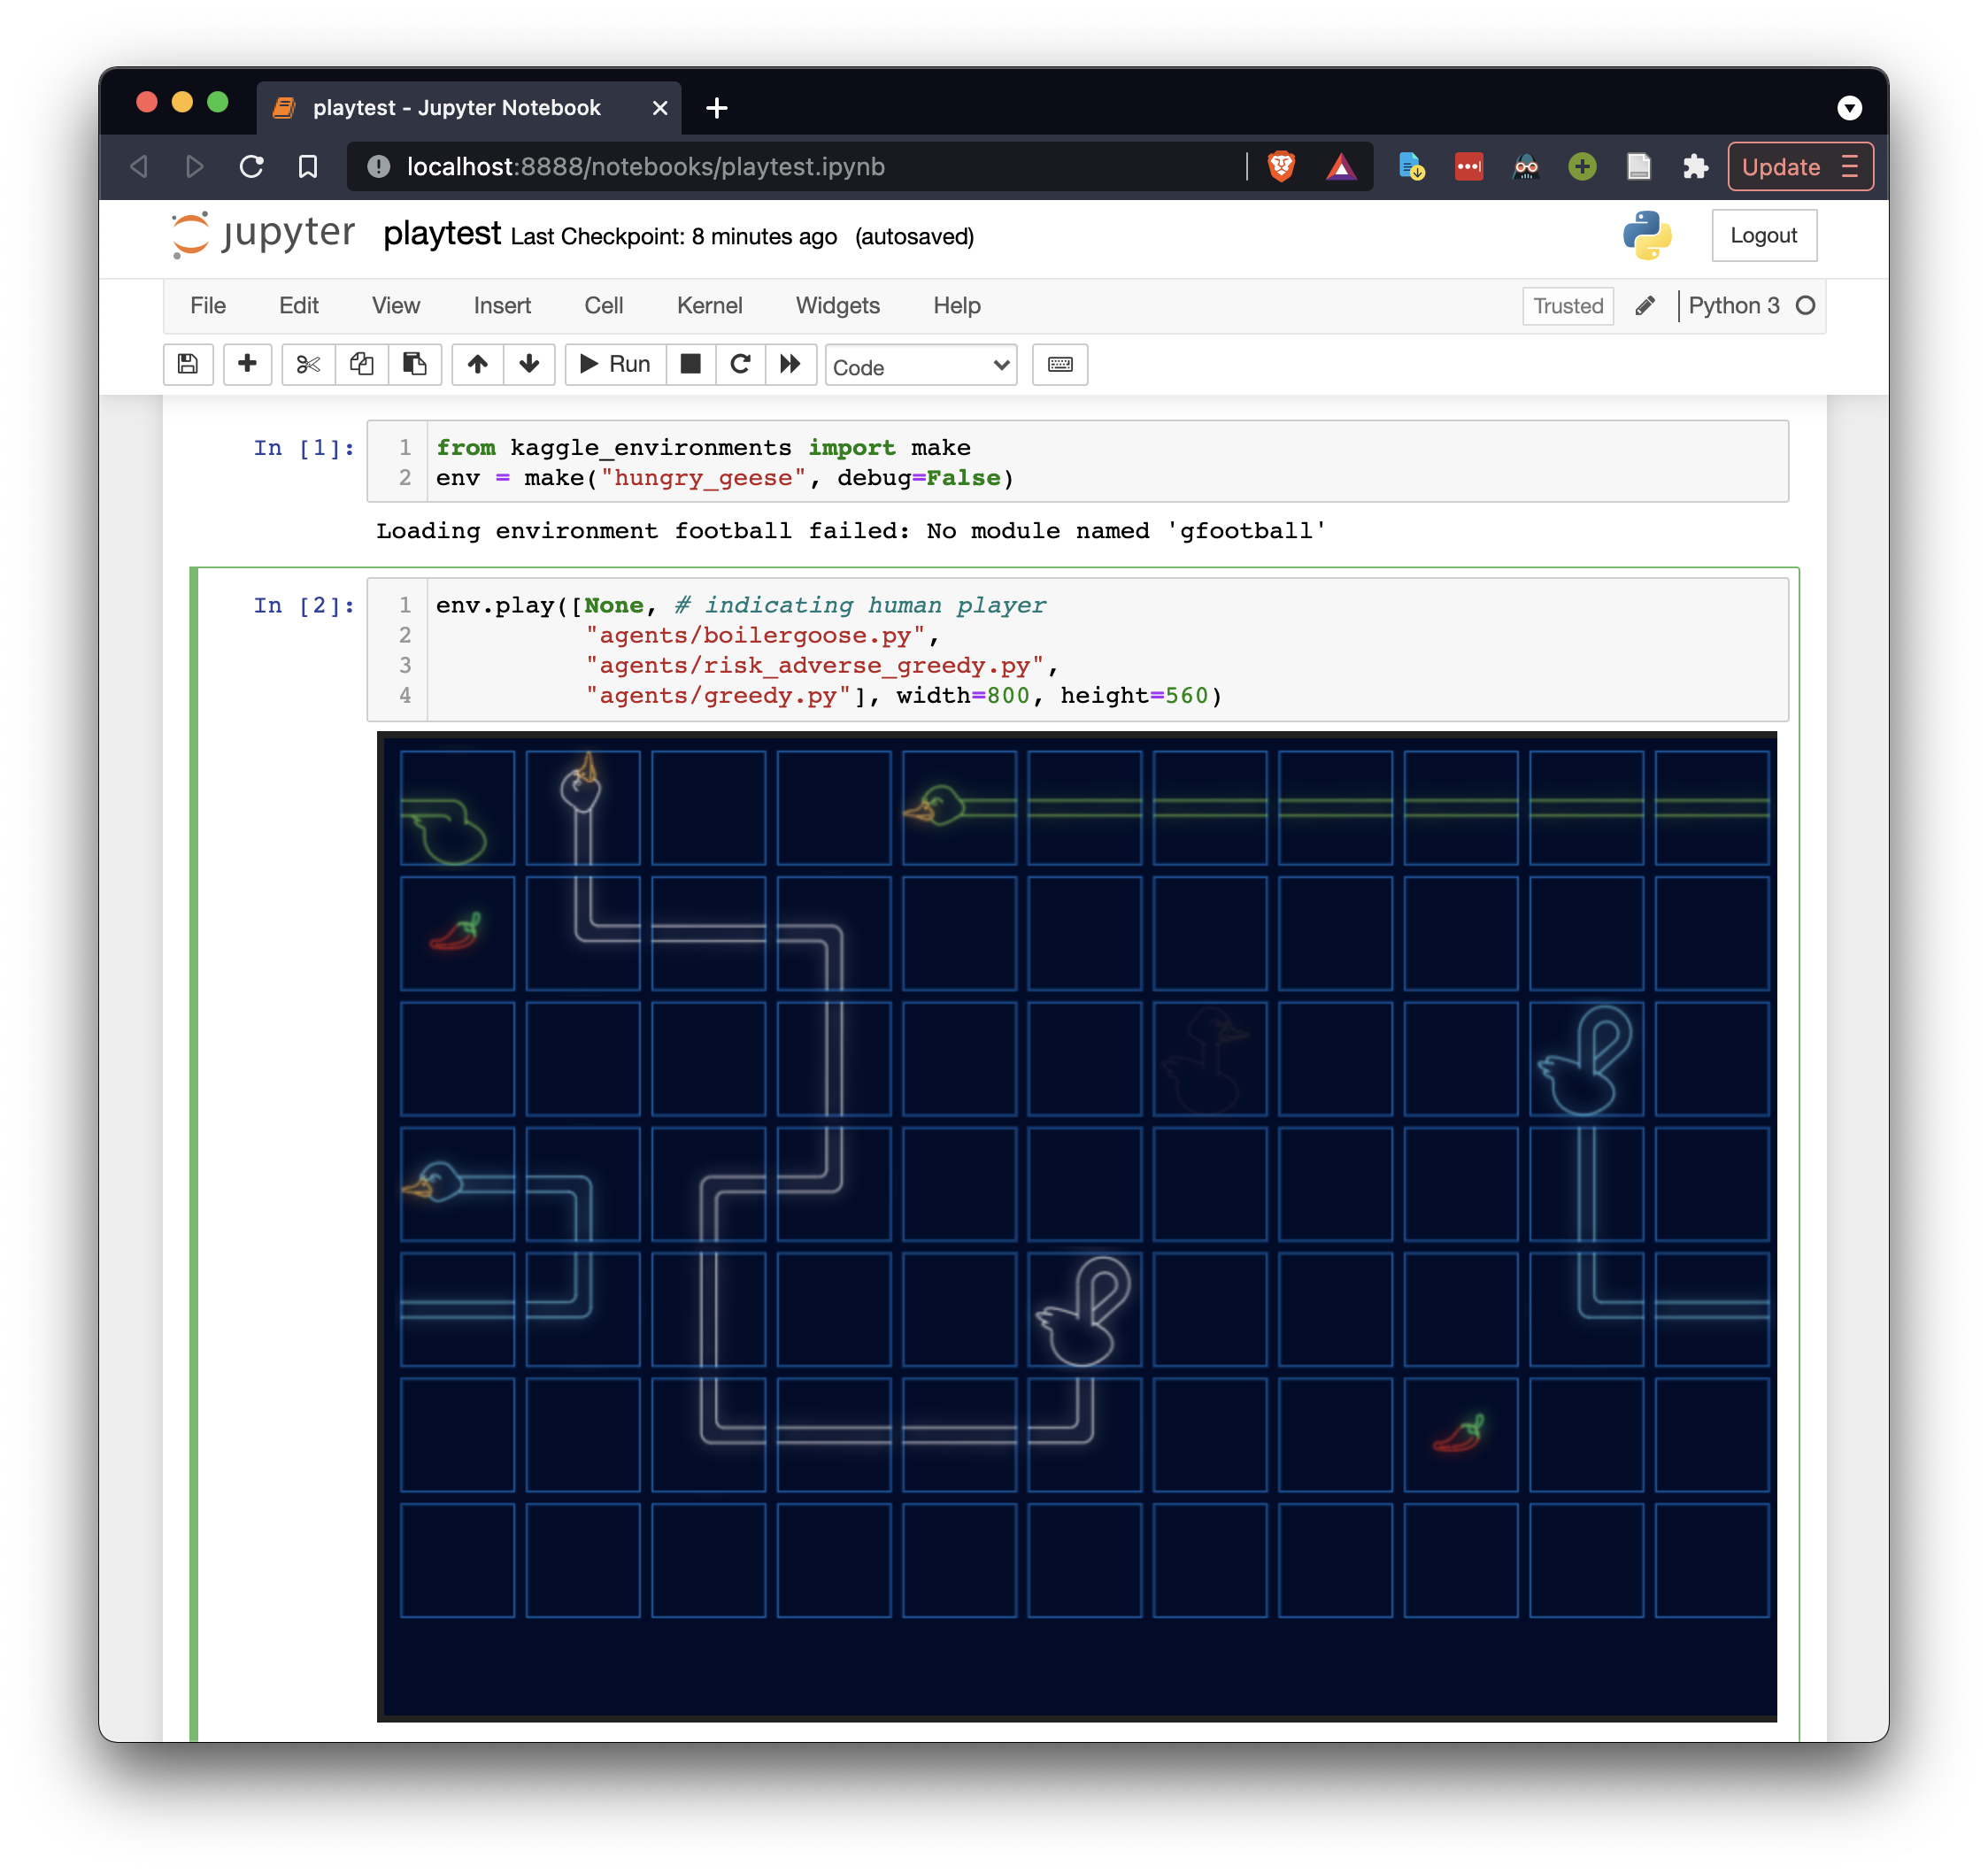
\includegraphics[width=0.95\textwidth]{images/notebook.png}
\caption{Screenshot of our GUI to play against the agents}
\label{figure_controls}
\end{figure}


% \newpage
% \begin{figure}[h]
% \centering
% \includegraphics[width=\textwidth]{images/root dir.png}
% \caption{Directory Hierachy in Jupyter Notebook after setup}
% \end{figure}

% \noindent Completing the above listed items allow you to start a local Jupyter Notebook with the local repository as the root directory as seen in Fig. X. We have provided a starter code within \verb|HumanPlayer.ipynb| illustrated in Figure 2.


When the game screen has loaded like what is seen in Figure \ref{figure_controls}, use your keyboard arrow keys (up, down, left, right) to move your agent. Your agent is the white goose.

You may choose to play against other agents by changing the arguments passed into \verb|env.play()| This list of agents are inside the \verb|./agents| folder. You may also add your own custom agent to play against. Playing against agents using Monte Carlo Tree Search is likely to be slow.

% We have configured the environment to keep playing until there is only one snake left, which would then be considered as the winner.

% \noindent Fig. X above shows the code to introduce a human player into the snake-game against other agents. To play against other types of agents, we can replace the list argument to \verb|env.play()| with a list of other agents while keeping one element as \verb|None| to represent the human player. At the moment, we only configured for 1 human player. Other types of agents are:

% %try to compress this into fewer lines?
% \begin{itemize}
%   \item \verb|boilergoose|
%   \item \verb|crazy_goose|
%   \item \verb|pubhrl|
%   \item \verb|pubhrl_latest|
%   \item \verb|risk_adverse_greedy|
%   \item \verb|simple_bfs|
%   \item \verb|simple_toward|
%   \item \verb|straightforward_bfs|
% \end{itemize}


% I have shown them together
% \section{GUI Code}
% \begin{figure}[h]
% \centering
% \includegraphics[width=\textwidth]{images/Human Player Code.png}
% \caption{Quickstart Code for Human Play}
% \end{figure}

% \begin{figure}[h]
% \centering
% 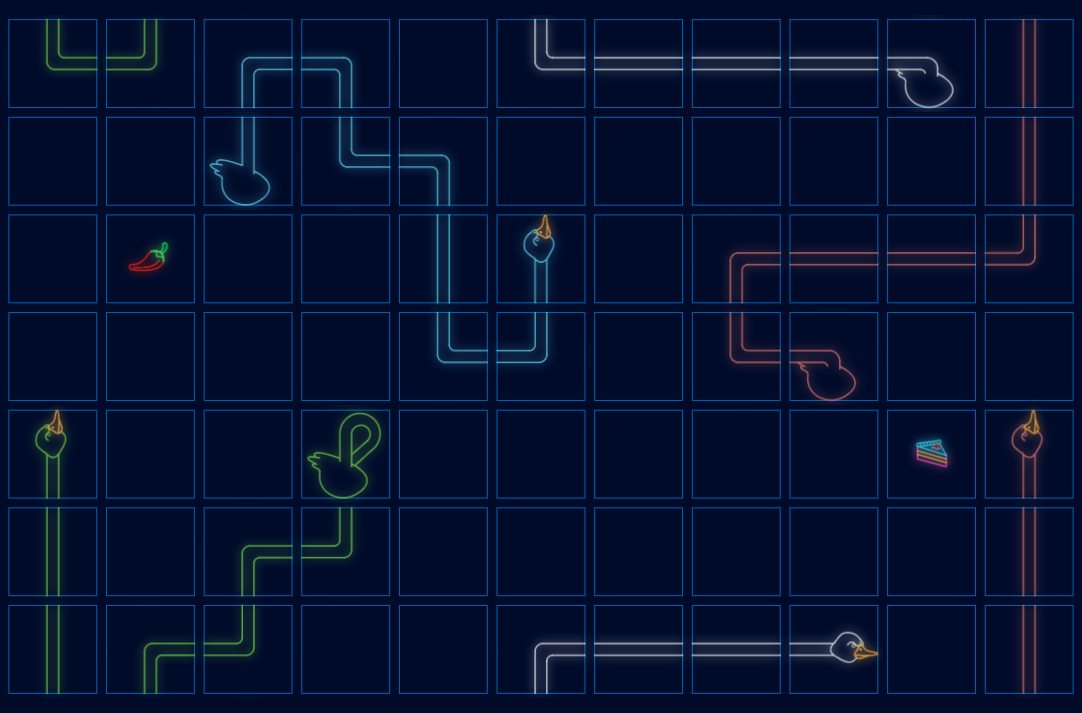
\includegraphics[width=\textwidth]{images/gameplay.png}
% \caption{Interactive Human Gameplay against loaded agents}
% \end{figure}

% \noindent Fig. X shows the step 10 of a current on-going game of a human player against 4 greedy agents. 


